\documentclass[12pt]{article}
\usepackage[landscape]{geometry}
\usepackage{amsmath}
\usepackage{tikz}

\begin{document}
\thispagestyle{empty}

\begin{minipage}[t]{0.6\textwidth}
{\large
\textbf{Professor: Brian Lins} \\
~\\
\textit{Spring 2024 Office Hours \& Class Schedule} 
}
\end{minipage}
%second column
\begin{minipage}[t]{0.4\textwidth}
\textbf{Office Location: Pauley 301} \\
\textbf{Office Phone: x6264} \\
\textbf{Email: blins@hsc.edu} \\
\end{minipage}

~
\begin{center}
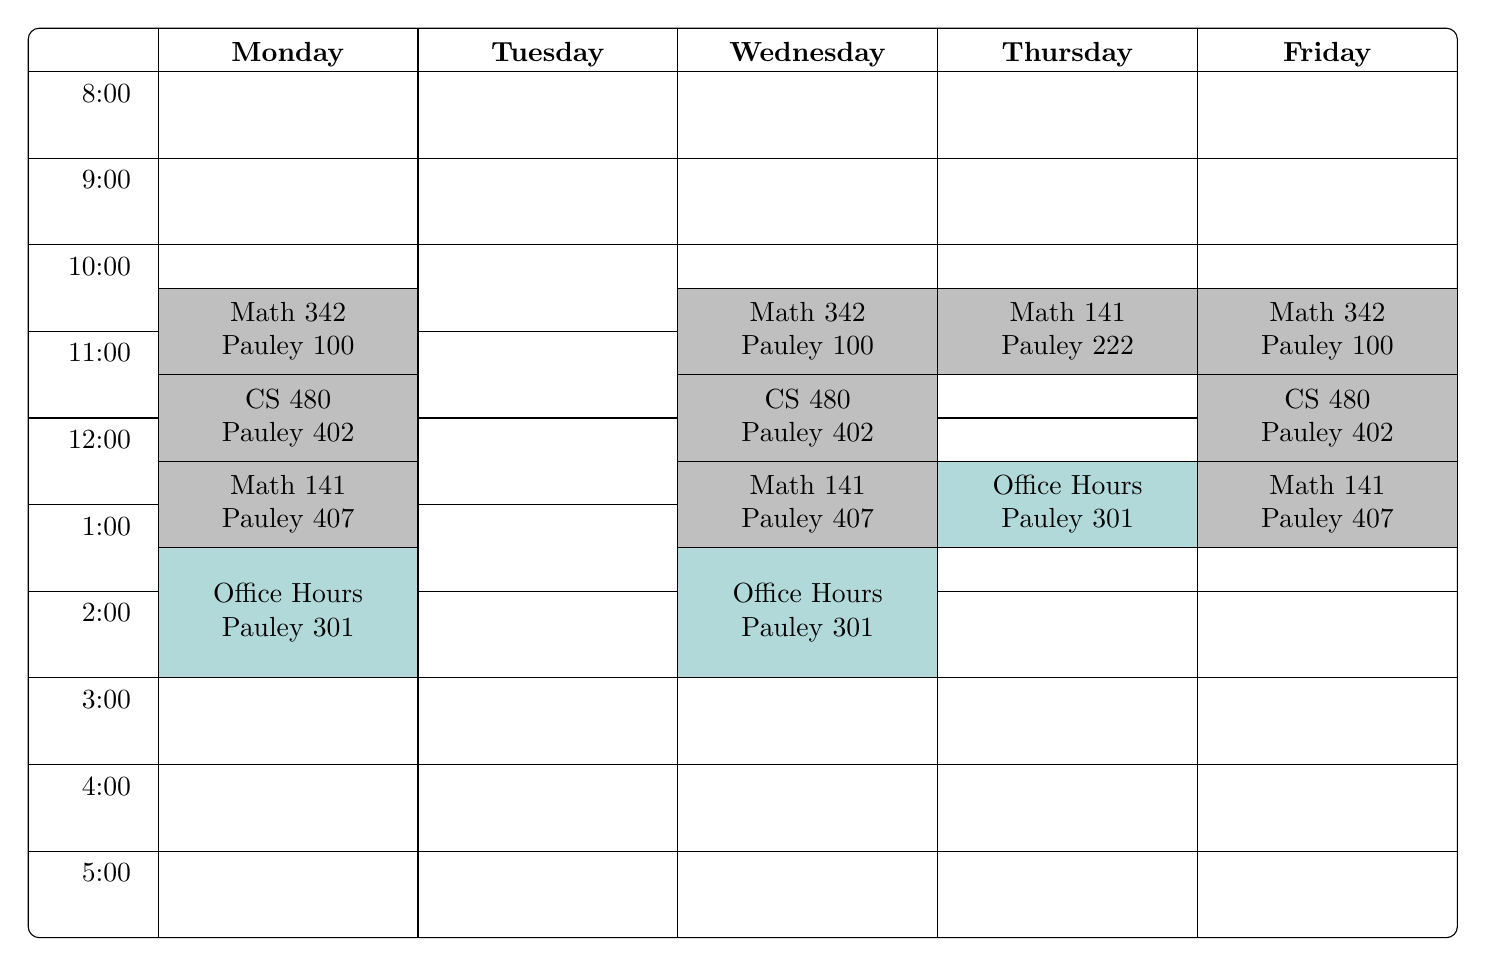
\begin{tikzpicture}[scale=1.1]
% border
\draw[rounded corners] (-1.5,10) rectangle (15,-0.5);

% rows
% main row separators
\foreach \i in {1,...,10} {
	\draw (-1.5,\i-0.5) -- (15,\i-0.5);
}
% times from 8 to 12
\foreach \i in {8,...,12} {
	\draw (-0.2,17-\i+0.25) node[left] {\i :00};
	%\draw (-0.2,17-\i-0.25) node[left] {\i :30};
}
% times from 1 to 5
\foreach \i in {1,...,5} {
	\draw (-0.2,5-\i+0.25) node[left] {\i :00};
}

% columns
% main column separators
\foreach \j in {0,...,4} {
	\draw (3*\j,-0.5) -- (3*\j,10);
}
\draw (1.5,9.7) node {\textbf{Monday}};
\draw (4.5,9.7) node {\textbf{Tuesday}};
\draw (7.5,9.7) node {\textbf{Wednesday}};
\draw (10.5,9.7) node {\textbf{Thursday}};
\draw (13.5,9.7) node {\textbf{Friday}};

% MWF Classes

\def\time{10.5};
\def\class{Math 342};
\def\room{Pauley 100};
\foreach \day in {1,3,5} {
	\filldraw[fill=gray!50] (3*\day-3,16.5-\time) rectangle (3*\day,17.5-\time);
	\draw (3*\day-1.5,17-\time) node {$\begin{array}{c} \text{\class} \\ \text{\room} \end{array}$};
}


\def\time{11.5};
\def\class{CS 480};
\def\room{Pauley 402};
\foreach \day in {1,3,5} {
	\filldraw[fill=gray!50] (3*\day-3,16.5-\time) rectangle (3*\day,17.5-\time);
	\draw (3*\day-1.5,17-\time) node {$\begin{array}{c} \text{\class} \\ \text{\room} \end{array}$};
}

\def\time{12.5};
\def\class{Math 141};
\def\room{Pauley 407};
\foreach \day in {1,3,5} {
	\filldraw[fill=gray!50] (3*\day-3,16.5-\time) rectangle (3*\day,17.5-\time);
	\draw (3*\day-1.5,17-\time) node {$\begin{array}{c} \text{\class} \\ \text{\room} \end{array}$};
}

% Thursday classes

\def\time{10.5};
\def\class{Math 141};
\def\room{Pauley 222};
\foreach \day in {4} {
	\filldraw[fill=gray!50] (3*\day-3,16.5-\time) rectangle (3*\day,17.5-\time);
	\draw (3*\day-1.5,17-\time) node {$\begin{array}{c} \text{\class} \\ \text{\room} \end{array}$};
}




% Monday & Wednesday Office Hours
\def\time{13.5};
\def\duration{1.5}
\def\class{Office Hours};
\def\room{Pauley 301};
\foreach \day in {1,3} {
	\filldraw[fill=blue!50!green!30!white] (3*\day-3,17.5-\duration-\time) rectangle (3*\day,17.5-\time);
	\draw (3*\day-1.5,17.5-\duration/2-\time) node {$\begin{array}{c} \text{\class} \\ \text{\room} \end{array}$};
}


% Thursday Office Hours
\def\time{12.5};
\def\class{Office Hours};
\def\room{Pauley 301};
\foreach \day in {4} {
	\filldraw[fill=blue!50!green!30!white] (3*\day-3,16.5-\time) rectangle (3*\day,17.5-\time);
	\draw (3*\day-1.5,17-\time) node {$\begin{array}{c} \text{\class} \\ \text{\room} \end{array}$};
}


% Friday Office Hours
%\def\time{9.0};
%\def\duration{1.0}
%\def\class{Office Hours};
%\def\room{Pauley 301};
%\foreach \day in {5} {
%	\filldraw[fill=blue!50!green!30!white] (3*\day-3,17.5-\duration-\time) rectangle (3*\day,17.5-\time);
%	\draw (3*\day-1.5,17.5-\duration/2-\time) node {$\begin{array}{c} \text{\class} \\ \text{\room} \end{array}$};
%}
%

\end{tikzpicture}
\end{center}

\end{document}
